%%%%%%%%%%%%%%%%%%%%%%%%%%%%%%%%%%%%%%%%%%%
%% Texto en ingles
%%%%%%%%%%%%%%%%%%%%%%%%%%%%%%%%%%%%%%%%%%%


This document presents an experimental validation of the test bench subsystem designed for the \textit{DAPHNE} boards that will be used in the DUNE experiment, specifically in the signal digitization phase. The methodology includes the procedures required to test simulated signals from neutrino events generated on FPGA-based hardware platforms. These signals are then converted to analog using an external DAC. The main steps of the experimental work are outlined below. % Este documento aborda una validación experimental del subsistema del banco de pruebas diseñado para las tarjetas DAPHNE que se utilizarán en el experimento DUNE, en particular en la fase de digitización de señales. La metodología incluye los procedimientos requeridos para probar señales simuladas de eventos de neutrinos generadas en plataformas de hardware basadas en FPGA. Posteriormente, estas señales se convierten en analógicas mediante un DAC externo. A continuación, se presentan los pasos principales del trabajo experimental.


    \subsection{Configuración del entorno experimental}
    
    El sistema experimental para las pruebas de generación de señales digitales, incluyen los siguientes componentes clave:
    \begin{itemize}
        \item Microcontrolador ESP32: Utilizado principalmente para aprovechar su DAC incorporado para procesar señales digitales generadas en un sistema externo al microprocesador. Este es programado con un FreeRTOS dedicado a las funciones de generación de eventos, tareas de adquisición y procesamiento mediante la plataforma de programación ESP-IDF (Espressif IoT Development Framework).
        
        \item Tarjeta de Desarrollo FPGA ARTY Z7 SoC Xilinx: Desde esta plataforma de hardware se realiza el diseño e implementación del sistema de generación de las señales digitales a procesar posteriormente.
        \item Analog Discovery 2: Instrumento utilizado para capturar la salida análogica generada mediante el DAC del microprocesador ESP32 y evaluar la fidelidad de la señal obtenida.
    \end{itemize}
    
    A continuación se observa un flujo de diseño de lo mencionado anteriormente.

    \vspace{0.3cm}

        \begin{figure}[H]
        \centerline{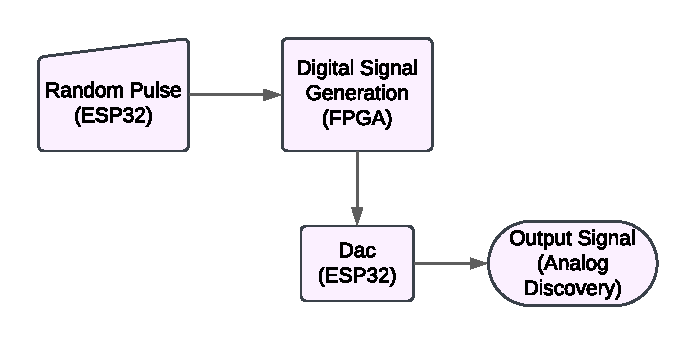
\includegraphics[scale=0.6]{montaje.pdf}}
        \caption{Flujo de diseño para la generación de señales digitales}
        \label{flujo_de_diseño}
        \end{figure}



    \vspace{0.3cm}
   \subsection{Generación y procesamiento de señales}
    
    Mediante el ESP32 se producen pulsos aleatorios simulando eventos de detección de neutrinos y desencadenando el envio de señales digitales implementadas dentro del diseño de hardware mediante protocolo de comunicación UART hacia el ESP32.
        
    Se modela en lenguaje de descripción de hardware (HDL) una señal característica (Fig.~\ref{modeled_neutrino}) correspondiente a la respuesta de un SiPM (Silicon Photomultiplier) frente a la radiación de centelleo generada por la interacción de neutrinos con átomos de argón líquido. Los SiPM son fotodetectores de alta sensibilidad que consisten en una matriz de diodos de avalancha interconectados, capaces de amplificar la corriente producida por la detección de fotones.

    La corriente generada por los SiPM pasa a través de una etapa de amplificación de transimpedancia antes de ingresar a un AFE (Analog Front-End). A partir de la función de transferencia correspondiente (Eq.~\ref{eq_z_neutrino}), se obtiene la señal modelada, característica de este tipo de sistemas de adquisición. Dicha señal alcanza una amplitud máxima proporcional a la cantidad de electrones generados en respuesta a la radiación detectada y presenta una caída exponencial que da lugar a la descarga y recuperación del estado inicial del sistema.

            \subsubsection{Datos Predefinidos} Se desarrolla una entidad en VHDL que transmite un flujo continuo de datos previamente generados mediante simulaciones que implementan técnicas de Montecarlo usando el software de simulación para detectores basados en Argón liquido LArSoft y herramientas de análisis como MATLAB \cite{SiPMmatlab}, el cuál considera las condiciones de operación del detector, la sección eficaz y la energía resultante de las particulas en la interacción \cite{LArSoft}. Esta señal simulada consta de un arreglo de 630 datos, con un valor máximo de 255, adaptado para el DAC de 8 bits del ESP32. Este conjunto de datos se denomina  \textit{datos RAW}.
            
            \subsubsection{Datos por Ecuación en Diferencias} Estas entidades en VHDL generan señales basadas en un modelo descrito mediante ecuaciones en diferencias. Inicialmente, se implementa una señal de decaimiento exponencial, representada por la Eq.~\ref{eq:exp}, junto con su correspondiente ecuación en diferencias (Eq.~\ref{eq:exp_dif}).
            
            A partir de los datos simulados con LArSoft, se modela la señal de detección de las interacciones utilizando una ecuación en tiempo continuo que representa de forma simplificada pero aproximada la respuesta típica de los SiPM como se muestra en la Fig.~\ref{modeled_neutrino} y la ecuación Eq.~\ref{eq_neutrino_time}. Posteriormente, se aplica un proceso de discretización mediante la transformada Z, generando el modelo que permita adaptarse para ecuaciones en diferencias que a su vez pueda ser implementada en el sistema embebido. En particular esta ecuación de diferencias corresponde a la función de transferencia de la señal preamplificada que ingresa al AFE. Este enfoque y representación de señales es comunmente usado en el diseño de filtros digitales, además el respectivo diseño de la señal de detección se desglosa como se muestra en el diagrama de la Fig.~\ref{eq_dif_schematic}.
        
    \subsection {Transmisión mediante protocolo UART y conversión Digital-Analoga}
        
        Se implementa una entidad en VHDL que se encarga exclusivamente de gestionar una máquina de estados finita (FSM) de dos estados para que los datos entrantes se serializen en cadenas de bytes que sean transmitidas a través de un pin GPIO hacia la tarjeta que incorpora el ESP32 al baudrate máximo establecido por la configuración estándar del receptor (1Mbits/s). El baudrate de comunicacion se obtiene a partir de un divisor de reloj basado en el reloj principal de funcionamiento del sistema. El estado llamado dentro del VHDL $S0_{init}$ recibe los datos entrantes, los concatena con 2 bits conocidos como de bits de parada y siempre y cuando este habilitada la comunicación serial por medio de un puerto entrante, la FSM transita al estado $S1_{Datos}$ que envia por cada flanco del reloj saliente del divisor cada bit que compone la cadena finalizando en los 2 bits de parada y despues retorna al estado inicial para reiniciar el proceso de envio con otra muestra.
        
        Los datos recibidos mediante UART se envian del buffer de recepción al DAC integrado en el microprocesador, el cuál tiene una resolución de 8 bits, generando señales analógicas en el rango de 0V a 3.3V (normalizado a 1V), monitoreando la salida análoga a través del Analog Discovery 2.        

    



%En esta etapa del desarrollo, se realizaron pruebas iniciales enfocadas en la frecuencia de operación para cada componente del sistema, específicamente en los DACs, asegurando que fueran alimentados con las frecuencias correctas. Estos avances reflejan resultados positivos en el manejo de las señales de frecuencia, destacando la capacidad de los sistemas para operar de manera estable y precisa.

%Además, se están desarrollando sistemas complementarios para caracterizar los experimentos, alineados con las metodologías empleadas por otros integrantes del equipo de trabajo, quienes se enfocan en el análisis de señales específicas. 


